\section{Die alljährliche Nikolaus-Aktion der Fachschaft Physik}
\begin{multicols}{2}
\textbf{HOHOHO, von drauß' vom Walde komm ich her\dots\
	mit Schokolade, was will man mehr?}

Alle Jahre wieder zur Vorweihnachtszeit habt ihr pünktlich zum Nikolaustag die Möglichkeit, euren Kommilitonen eine kleine, süße Freude zu bereiten. Genauer gesagt könnt ihr ihnen einen Schokonikolaus mit Grußkärtchen schenken. 
Die Nikoläuse werden dann "stilecht" vom Nikolaus (oder eher Weihnachtsmann) und seinen Engeln in den Grundvorlesungen verteilt.

Dadurch habt ihr die perfekte Möglichkeit, besonderen Menschen zu zeigen, dass ihr sie mögt. Oder alternativ auch als Dankeschön für die ein, zwei zugestellten Übungsaufgaben, als Motivationshilfe, unauffälliger Flirtversuch oder um die Vorlesung für eine Weile zu unterbrechen. Es wurde auch schon dadurch dem ein oder anderem Prof für eine gute Vorlesung gedankt und man munkelt, dass vereinzelte Grußkärtchen in deren Büros aufzufinden sind und dort stetig zu einer guten Laune beitragen. ;)

Die Nikolaus-Aktion wird immer rechtzeitig vorher in den Vorlesungen angekündigt. So habt ihr die Möglichkeit, rechtzeitig in der Fachschaft euer Grußkärtchen zu erwerben und kreativ zu gestalten. 

Verteilt werden die Nikoläuse mit den Grußkärtchen am 6.~Dezember in den jeweiligen Pflichtmodule des ersten, dritten und fünften Semesters. Das bedeutet entweder in der Mathe- oder Physik-Vorlesungen (je nachdem, welche gerade an dem besagten Tag ist).
2-Fach-Bachelor müssen ein wenig aufpassen, wenn die Nikoläuse in einer Mathe-Vorlesung verteilt werden.
Sollte die beschenkte Person nicht in der Vorlesung anwesend sein, kann sie den Nikolaus noch einige Tage im Raum der Fachschaft abholen.
Fällt der 6.~Dezember auf ein Wochenende, werden die Nikoläuse am folgenden Vorlesungstag von uns ausgeteilt.

Auf eine schöne Vorweihnachtszeit, euer Nikolausteam!

\fibelsig{Miriam N.}
\end{multicols}

\vspace{\fill}
\begin{center}
	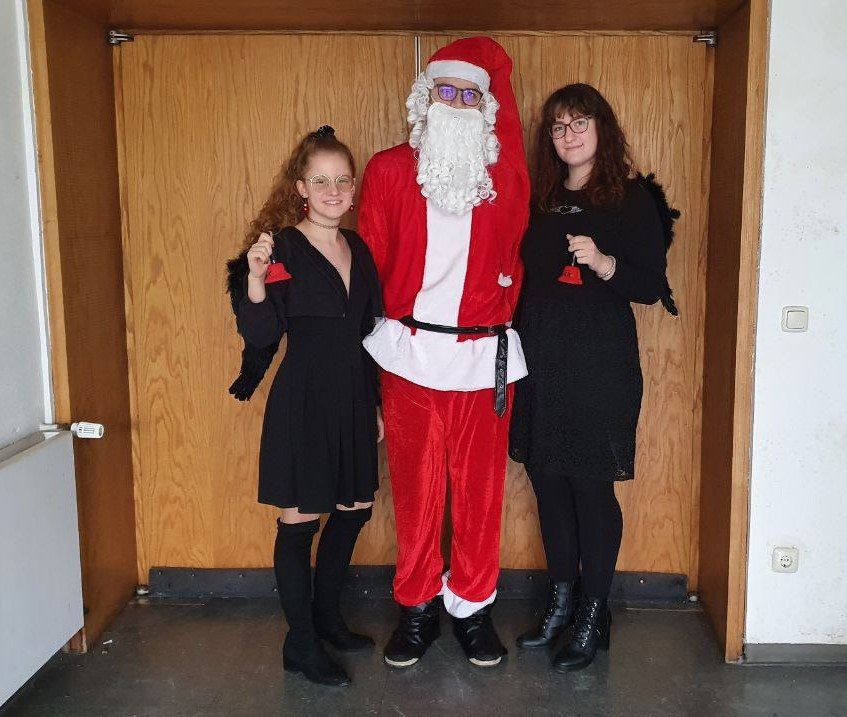
\includegraphics[width=0.8\textwidth]{res/Nikoklaus_cut.jpg}
\end{center}
